\documentclass[c5size]{ctexart}
\usepackage{lipsum} %生成随机文本
\usepackage{ctex} %中文包
\usepackage[colorlinks=true]{hyperref} %设置交叉引用
\usepackage[left=2cm, right=2cm, top=3cm, bottom=3cm]{geometry} %设置页面布局
\usepackage{amsmath} %数学包
\usepackage{apacite} %参考文献设置为APA格式
\usepackage{graphicx} %导入图片
\usepackage{listings} %插入代码
\usepackage{xcolor}
\pagestyle{headings}
\usepackage{booktabs}
\lstset{
	%行号
	numbers=left,
	%背景框
	framexleftmargin=10mm,
	frame=none,
	%背景色
	%backgroundcolor=\color[rgb]{1,1,0.76},
	backgroundcolor=\color[RGB]{245,245,244},
	%样式
	keywordstyle=\bf\color{blue},
	identifierstyle=\bf,
	numberstyle=\color[RGB]{0,192,192},
	commentstyle=\it\color[RGB]{0,96,96},
	stringstyle=\rmfamily\slshape\color[RGB]{128,0,0},
	%显示空格
	showstringspaces=false
}

\title{基于深度强化学习和蒙特卡洛搜索树的连六棋AI}
\author{江俊广(2015011584)、陈宇韶(2015012182)、郑洛成(2015011626)}
\date{\today}

\begin{document}
	\maketitle

\section{Introduction}
	五子棋是世界智力运动会竞技项目之一,是一种两对弈的纯策略型棋类游戏,玩家双方分别使用黑白两子,下在棋盘直线与横线的交叉点上,先连成五子(五子在一条横线、竖线或对角线上)的玩家获胜。一方面,五子棋容易上手,难度小于围棋;另一方面,五子棋具有一定的策略性,需要玩家具有一定技巧。所以五子棋实现的时候工程量适合大作业制作周期。\par
	我们在Github上已经找到了类似于AlphaZero原理的五子棋AI——AlphaZero-Gomoku。其框架可以作为我们的参考。\par
	
	然而,五子棋本身规则具有一定缺陷。首先,实际比赛中五子棋先后手优势差距比较大,先手往往能够决定胜局,所以历史上各国的棋手们采取一系列方法限制先手的优势来达到平衡先后手的目的,但仍然不能够很好解决问题,同时容易导致规则过于复杂。如禁手规则实行之后仍然会导致“先手必胜”。而基于“连珠棋”思路的RIF规则、Sakata规则、Yamaguchi规则和Tarannikov规则将禁手、交换、缩小棋盘的思维结合,虽然可以平衡优势,但规则复杂,降低游戏可玩性,且先后手的公平性仍然无法严格保证。\par
	
	AlphaZero-Gomoku基于无禁手的规则,但是在实际运行中出现的问题是,后手人类比较难战胜先手AI,后手AI也比较难战胜先手人类。所以我们考虑更改五子棋为连六棋,即连成六子获胜。持黑者第一手放一个黑子于棋盘上,之后双方轮流著手,每手放二个棋子于棋盘上。这样可以保证游戏的公平性,因为各方每次下完一手后,盘面都比对方多一子,因此赛局可自然达成平衡的状态,这使得公平性大为提升。另外六子棋不具有先手优势。所以也不需要为了保持公平性,而制定一些额外的规则。理论上游戏所使用的棋盘可以是无限大的。对一般玩家而言,采用围棋的十九路棋盘即可。\par
	
\section{不同算法及其优劣的比较}
\subsection{极小极大搜索}
	假设有两个玩家MIN和MAX,给定一棵博弈树,最优策略可以通过检查每个节点的极大极小值来决定,这里我们记为MINIMAX-VALUE(n)。假设在某一步以后两个游戏者都按照最优策略进行,那么这一个节点的极小极大值就是对应状态的效用值。显然对于终止状态,极小极大值就是它的效用值。此外,已知一个选择,MAX将优先选择移动到一个有极大值的状态,而MIN选择移动到有极小值的状态。所以我们得到如下公式:
	
	\begin{align}
		MINIMAX-VALUE(n) = 
		\begin{cases}
		UTILITY(n),\text{当n为终止状态}\\
		max_{s \in Successor(n)}MINIMAX-VALUE(s),\text{当n为MAX节点}\\
		min_{ s \in Successor(n)} MINIMAX-VALUE(s),\text{当n为MIN节点} \\
		\end{cases}
	\end{align}
	
	该算法从当前状态计算极小极大决策,它使用了简单的递归算法,计算每个后继的极小极大值,直接实现定义公式。递归算法自上而下一直前进到树的叶节点,然后随着递归回溯,通过树把极小极大值回传。极小极大值对博弈树执行了一个完整的深度优先搜索。如果树的最大深度是m,在每个节点的合法招数有b个,那么极小极大算法的时间复杂度是$O(b^m)$。对于一次性生成所有的后继节点的算法,空间复杂度是$O(b^m)$,而对于每次生成一个后继的算法,空间复杂度是$O(m)$。然而对于真实的游戏,这样的时间开销完全不实用。
	
\subsection{alpha-beta剪枝算法}
	极小极大值搜索的问题必须检查游戏状态的数目随着招数的数量指数级增长。我们没有办法消除这种指数级增长,不过我们可以通过剪枝将其有效减半。我们有可能不需要遍历博弈树中每一个节点就可以计算出正确的极小极大值策略。\par
	
	alpha-beta剪枝可以用于树的任何深度,而且很多情况下可以剪裁整个子树,而不是仅仅剪裁叶节点。一般原则是:考虑树中某处的节点n,游戏者可以选择移动到该节点。如果游戏者在n的父节点或者更上层的任何选择点有一个更好的选择m,那么在实际的游戏中就永远都不会到达n。所以一旦我们发现关于n的足够信息(通过检查它的某些后代),就可以得到上述结论,我们就可以剪裁它。\par
	
	因为极小极大搜索是深度优先的,所以任何时候我们不得不考虑树中一条单一路径上的节点以选取参数alpha和beta。其中,\par
	alpha = 到目前为止我们在路径上的任意选择点发现的MAX的最佳(即极大值)选择\par
	beta = 到目前为止我们在路径上的任意选择点发现的MIN的最佳(即极小值)选择\par
	alpha-beta搜索不断更新alpha和beta的值,并且当某个节点上的值分别比目前的MAX的alpha或者MIN的beta值更差的时候剪裁这个节点剩下的分支(即终止递归调用)。\par
	
	alpha-beta剪枝的效率很大程度上取决于检查后继的顺序,如果我们能够做到先检查那些最好的后继,那么alpha-beta算法只需检查$O(b^(d/2))$个节点来决定最佳招数,而极小极大值算法需要检测$O(b^d)$。这意味着有效分支因子由b变成了$\sqrt{b}$。在相同的时间里,alpha-beta算法能够比极小极大值算法多向前预测大约两倍的步数。如果后继者不是按照最佳优先的顺序,而是按照随机的顺序检查的,那么对于适当的b,要检查的总节点数大约是$O(b^(3d/4)$。\par
	
	对于双人博弈游戏,极小极大值算法以及其改进后的alpha-beta剪枝算法比较依赖于当前棋盘状态相关的效用函数。当效用值的节点不是最终节点时,效用函数往往来自于人为编写的专家系统,而专家系统的优劣直接决定了效用函数的准确度。不准确的效用函数会舍去一些合理的决策分支,使博弈结果不理想。\par
	
\subsection{蒙特卡洛树搜索算法}
	蒙特卡洛树搜索算法通过对随机的游戏进行推演来逐渐建立一棵不对称的搜索树步骤大致可以分为选择(Selection),拓展(Expansion),模拟(Simulation),反向传播(Backpropagation)四步。
	
	选择阶段需要从决策的局面R出发向下选择出一个最急迫需要被拓展的节点N。如果所有的可行行动都已经被拓展过了,那么使用上置信公式计算该节点所有子节点的置信上界(UCB),找到值最大的子节点继续检查。反复向下迭代。如果被检查的局面依然存在没有被拓展的子节点,那么我们认为这个节点就是本次迭代的目标节点N,找出N还未被拓展的动作A,执行拓展操作。如果被检查的节点是一个游戏已经结束的节点,那么从该节点直接执行反向传播。
	
	拓展阶段时,在搜索树中创建一个新的节点Nn作为N的一个新子节点。Nn的局面就是节点N在执行了动作A后的局面。
	
	在模拟阶段,从Nn开始,让游戏随机进行,直到得到一个游戏结局,来作为Nn的初始评分。以胜利/失败来评分,分别为1和0。
	
	反向传播阶段,节点N以及从根节点到N的路径上的所有节点都会根据本次模拟的结果来添加自己的累积评分。如果选择阶段直接发现了一个游戏结局,根据该结局来更新评分。
	每一次迭代都会拓展搜索树,当到了一定的迭代次数或者时间之后结束,选择根节点下最好的子节点作为本次决策的结果。
	
	随机性过强时,蒙特卡洛树搜索算法会使资源浪费到不需要考虑的状态空间中,因此,很多著名的棋类AI系统(如fuego,Mango,AlphaGo )在运用蒙特卡洛树搜索时都会进行剪枝,从而使计算资源更多地分布到合理的对弈策略中。
	
	此外,双人游戏博弈中蒙特卡洛树搜索并不一定能够收敛到最优解的情况,因此需要对其进行改进。
	
\subsection{深度强化学习算法+蒙特卡洛搜索树算法}
	由于蒙特卡洛树搜索算法随机性强,计算成本过高,为了改进搜索策略,我们向蒙特卡洛树搜索算法中引入深度强化学习算法。
	
	深度学习是机器学习中建模数据的隐含分布的多层表达的算法。换句话说,深度学习算法自动提取分类中所需要的低层次或者高层次特征。因此深度学习能够更好的表示数据的特征,同时由于模型的层次、参数很多,容量也足够,因此,深度学习模型有能力表示大规模数据。
	强化学习是一个连续决策的过程,其特点是不给任何数据做标注,仅仅提供一个回报函数,这个回报函数决定当前状态得到什么样的结果(比如“好”还是“坏”),从数学本质上来看,还是一个马尔科夫决策过程。强化学习最终目的是让决策过程中整体的回报函数期望最优。
	
	我们可以使用自我对局不断训练更新当前最新的模型,模型训练好之后,仍然用蒙特卡洛树搜索算法,继续让机器进行自我对局,只不过把投子的策略,从均等概率的随机投子,改为根据训练得到的模型的指导,来决定下一手的投子位置。具体操作是根据当前棋面,估算下一手的投子位置,每一个位置的赢率和投子概率不同,赢率和投子概率越高,得分越高。
	
	但仅仅靠此方法生成的数据多样性不强,因此强化学习算法中一般会特意设计探索手段,如使用置信上限来鼓励探索新的投子位置,越是以往很少投子的位置,UCB得分越高。
	
	因此可以综合考虑下一手棋面的赢率、投子概率和UCB来给下一手各个投子位置打分,取其中得分较高者来指导蒙特卡洛树搜索算法,决定下一个投子的位置。用改进了投子策略的蒙特卡洛树搜索算法,让机器继续自我对弈,这样得到更多棋谱,然后用这些棋谱再次训练模型,提高赢率和投子概率的估算精度,如此循环重复,不断提高精度。
	
\section{不同游戏规则及其学习策略的比较}
\subsection{围棋与alpha zero}
	围棋使用方形格状棋盘及黑白二色圆形棋子进行对弈,棋盘上有纵横各19条线段将棋盘分成361个交叉点,棋子走在交叉点上,双方交替行棋,落子后不能移动,以围地多者为胜。因为黑方先走占了便宜,所以人为规定黑方局终时要给白方贴子。中国古代围棋是黑白双方在对角星位处各摆放两子(对角星布局),为座子制,由白方先行。现代围棋由日本发展而来,取消了座子规则,黑先白后,使围棋的变化更加复杂多变。围棋也被认为是世界上最复杂的棋盘游戏。\par
	
	alpha zero使用自我对局来进行训练,不断更新新模型,并且只保留新模型。每一个self-play对局的前30步,action是根据正比于蒙特卡洛树搜索根节点处每个分支的访问次数的概率采样得到的,之后的exploration则是通过直接加上Dirichlet noise的方式实现的。\par
	
	self-play收集到的数据就是用来训练策略价值网络的,而训练更新的策略价值网络也会马上被应用到蒙特卡洛树搜索中进行后面的self-play,以生成更优质的self-play数据。两者相互嵌套,相互促进,就构成了整个训练的循环。\par
	
\subsection{五子棋与github上已经找到的算法框架}
	AlphaZero-Gomoku基本上采用了AlphaZero的算法框架,为了能够在算力非常弱的情况下尽快的收集数据训练模型,每一局self-play结束后,该算法框架会把这一局的数据进行旋转和镜像翻转,将8种等价情况的数据全部存入self-play的数据缓存中。这种旋转和翻转的数据扩充在一定程度上也能提高self-play数据的多样性和均衡性。
	
\subsection{连六棋与我们的实现}
	\subsubsection{规则的改变和公平性的保证}
		连六棋改变了游戏规则,除了将获胜条件由五连子改为六连子之外,还有第二手及之后每一手投两个子。这样可以保证游戏的公平性,因为各方每次下完一手后,盘面都比对方多一子,因此赛局可自然达成平衡的状态,这使得公平性大为提升。另外六子棋不具有先手优势。所以也不需要为了保持公平性,而制定一些额外的规则。
		
	\subsubsection{蒙特卡洛搜索树的调整}
		\paragraph{调整原因}
			连六棋每一回合可以走两个棋子,因此走法复杂度是相同规模的五子棋的走法复杂度的平方,尽管搜索树的深度变成了原先的一半。更大的问题是神经网络的输出表示变得比较复杂,原先用棋盘大小的概率矩阵表示,现在必须用$\text{棋盘大小}^2$的概率矩阵表示。
		\paragraph{解决方法}采用贪心决策,即每一回合的每步都选尽可能是当前局面最优的棋子。AI在棋盘上选择一个棋子后,基于新的棋盘再选择一个棋子。尽管不能保证两步结合后一定是最优决策,但是不会太差,同时可以使得走法复杂度降低一个平方数量级,同时使得神经网络的输出较为简洁。
		\paragraph{具体修改}修改蒙特卡洛搜索树的树节点,原先是父子结点代表两个对手,现在是爷爷和孙子节点代表两个对手,在从叶节点向上传递局面评估值的时候需要判断何时取反。
	\subsubsection{神经网络输入的调整——棋盘状态的表示}
		AlphaGo Zero中,一共使用了17个二值特征平面来描述当前局面,其中前16个平面描述了最近8步对应的双方player的棋子位置,最后一个平面描述当前player对应的棋子颜色,即先后手
		
		五子棋用“4个的二值特征平面”表示,其中前两个平面分别表示当前player的棋子位置和对手player的棋子位置,有棋子的位置是1,没棋子的位置是0. 然后第三个平面表示对手player最近一步的落子位置,也就是整个平面只有一个位置是1,其余全部是0. 第四个平面,也就是最后一个平面表示的是当前player是不是先手player,如果是先手player则整个平面全部为1,否则全部为0。
		
		连六棋用4个二值特征平面表示,前两个平面分别表示当前player的棋子位置和对手player的棋子位置,有棋子的位置是1,没棋子的位置是0。第三个平面表示对手player最近一回合下的所有棋子, 整个平面最多2个1,其余全部是0。第四个平面表示当前player在该回合已经下的棋子,整个平面最多1个1,其余全部是0。由于连六棋中,先后手并没有什么太大的区别,因此去除了五子棋中表示先后手的平面。

\section{实验结果与分析}
	\subsection{损失函数与熵值函数的变化趋势}
		六子棋的训练目标达到与否使用损失函数loss以及熵entropy描述。通过策略价值网络,即给定当前局面s的情况下,返回当前局面下一个可行的action的概率以及当前评分的模型。我们在self-play的过程中收集一系列的(s,$\pi$,z)数据。其中s是当前局面的描述,由四个width×height矩阵表示,第一个矩阵表示所有我方的棋子,第二个矩阵表示所有对方的棋子,第三个矩阵表示对方在上一回合下的所有棋子,第四个矩阵表示我方在该回合已经下的棋子;$\pi$是蒙特卡洛树搜索输出的概率;z是真实的对局结果:使用1表示当前玩家获胜,0表示平局,-1表示对方玩家获胜。我们训练的目标是让网络输出action的概率p更加接近蒙特卡洛树搜索输出的概率$\pi$,让网络输出的局面评分v能更准确地预测真实的对局结果z。从优化的角度讲,我们是在self-play的数据集上不断地最小化损失函数:
		\begin{equation}
			l = (z-v)^2-\pi ^T\log P + c\Arrowvert \theta \Arrowvert ^ 2
		\end{equation}
		其中第三项是为了防止过拟合的正则项。我们进行了两次训练,在最后一次训练过程中,损失函数的变化如下所示:
		\begin{figure}
			\caption{损失函数随训练局数的变化}
			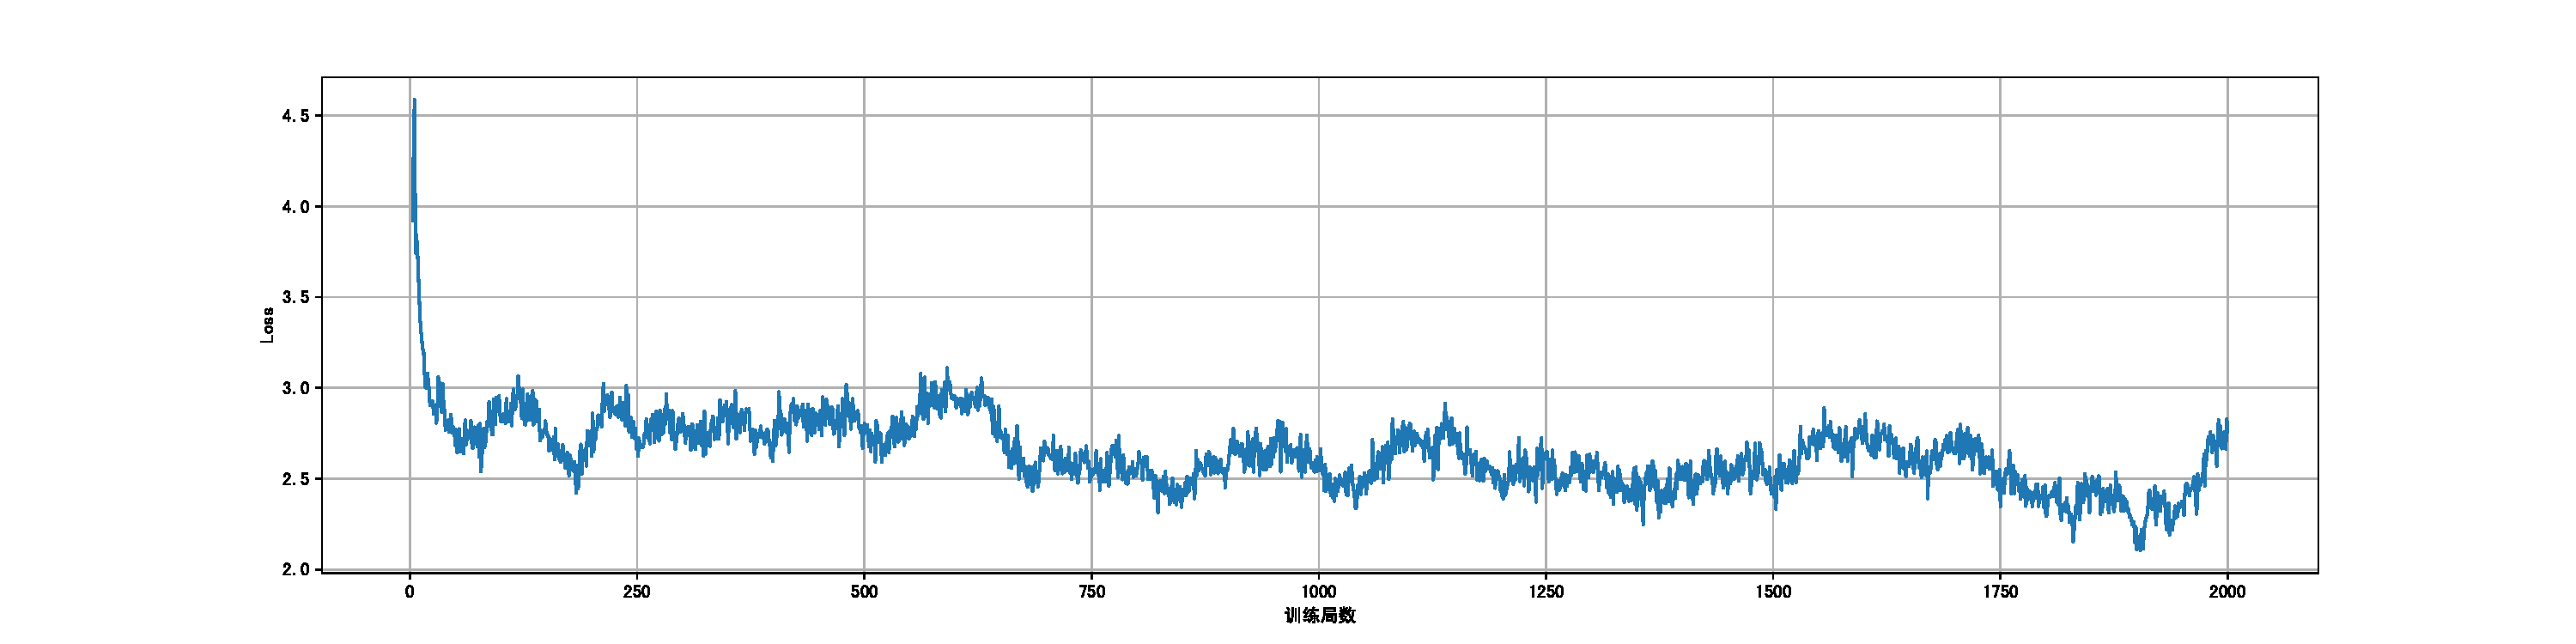
\includegraphics[scale=0.4]{Loss.pdf}
			\label{fig:Loss}
		\end{figure}
		从图\ref{fig:Loss}可以观察到前100局损失函数迅速到3.0以下,随后直到训练到第1750局损失函数在[2.5,3]之间波动,同时数值略有下降,到大约1900局时损失函数降低到训练次数范围的最低点,之后出现上升。根据变化的总体趋势,我们推测损失函数正在随着训练次数的增加缓慢下降,1900局之后的上涨是损失函数的波动所致。长远来看,在训练到一定的局数后损失函数仍会重新下降。\par
		除了损失函数以外,我们还关注落子概率分布的熵值entropy的变化情况。正常来讲,在开始的时候,我们的网络会随机输出落子的概率,所以熵值较大,随着训练结果慢慢推进,网络会慢慢学会在不同的局面下哪些位置会有更大的落子概率,此时落子概率的分布不再均匀,而是有较强的偏向,这样entropy的值就会变小。由于输出的偏向,才能帮助蒙特卡洛树搜索在搜索过程中在更有潜力的位置进行更多的模拟,从而在较少的模拟次数下达到比较好的性能,图\ref{fig:Entropy}是最后一次训练时观察到的entropy变化情况:
		\begin{figure}
			\caption{熵随训练局数的变化情况}
			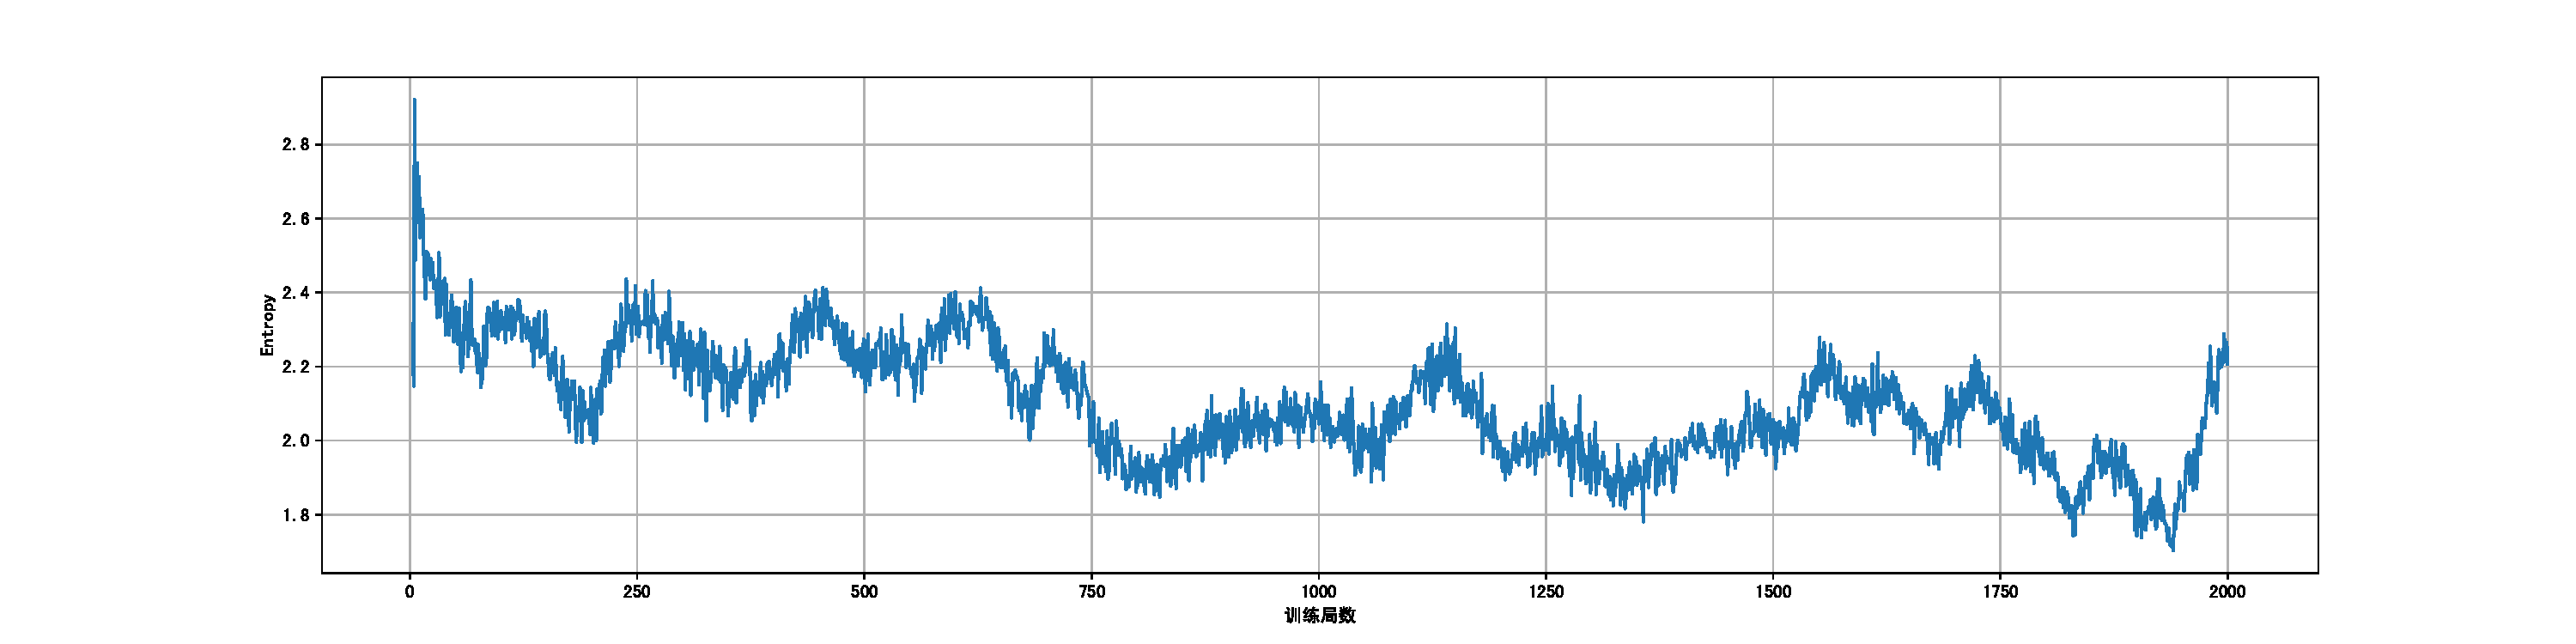
\includegraphics[scale=0.4]{Entropy.pdf}
			\label{fig:Entropy}
		\end{figure}
		由图\ref{fig:Entropy}可见,entropy大体上随着训练局数的增加逐渐减小,在前200局entropy的下降最快,从大约2.9下降到2.0,之后entropy出现波动,但波动极大值与极小值均有下降,并在大于1900局熵值达到最低,之后熵值回升,我们推测熵值回升属于波动的过程,长远来看,总体趋势仍是下降。
		
	\subsection{AI对战的测试结果}
		为了更为直观地衡量AI的训练效果,我们采用对战评估的方式,即让我们的AI与采取不同算法的AI进行对战,测试胜率来判断训练效率以及AI战力是否达到预期。采取不同算法的AI分别有纯蒙特卡洛树搜索的AI 。此外,我们还测试了人类与AI对战来更为判断我们的AI的战力是否足够优秀。
		\subsubsection{连六棋AI vs. 纯蒙特卡洛树搜索的AI}
			第一次训练的连六棋AI与采用纯蒙特卡洛树搜索的AI对战结果如表\ref{table:train_result1}所示,其中胜率采用对阵10次的连六棋AI胜率,纯蒙特卡洛树搜索AI的战力表示模型每一步使用模拟次数:
			\begin{table}[!htbp]
				\centering
				\caption{第一次训练的连六棋AI与采用纯蒙特卡洛树搜索的AI对战结果}
				\label{table:train_result1}
				\begin{tabular}{lll}
					\toprule
					Self-play 次数 & pure\_MCTS战力 &胜率 \\
					\midrule
					50          & 1000             & 0.3 \\
					100         & 1000             & 0.8 \\
					150         & 1000             & 0.9 \\
					200         & 1000             & 0.7 \\
					250         & 1000             & 1.0 \\
					300         & 2000             & 0.8 \\
					350         & 2000             & 0.7 \\
					400         & 2000             & 0.9 \\
					450         & 2000             & 0.8 \\
					500         & 2000             & 1.0 \\
					550         & 3000             & 0.8 \\
					600         & 3000             & 1.0 \\
					650         & 4000             & 1.0 \\
					700         & 5000             & 0.9 \\
					750         & 5000             & 0.9 \\
					800         & 5000             & 0.9 \\
					850         & 5000             & 1.0 \\
					900         & 6000             & 0.9 \\
					950         & 6000             & 0.7 \\
					1000        & 6000             & 0.8\\
					\bottomrule
				\end{tabular}
			\end{table}
		从表\ref{table:train_result1}中可以看出,与相同战力的纯蒙特卡洛树搜索AI相比较,self-play次数越多连六棋AI的胜率越高,甚至可以达到1.0的胜率。更高战力的纯蒙特卡洛树搜索AI仍可用更多次self-play的连六棋AI超越。与相同战力的纯蒙特卡洛树搜索AI对战时,self-play次数增加时胜率出现一段下降的区间,胜率的波动可能来源于loss function与entropy的波动,也可能来源于测试局数较少导致的偶然因素。Self-play的次数小于纯蒙特卡洛树搜索的每步模拟次数,说明连六棋AI的训练效率相比纯蒙特卡洛树搜索有了显著的改进,达到同样效果所需的资源更少。改进之后进行第二次训练,得到了更强的AI,对战结果如表\ref{table:train_result2}所示:
		
			\begin{table}[!htbp]
				\centering
				\caption{第二次训练的连六棋AI与采用纯蒙特卡洛树搜索的AI对战结果}
				\label{table:train_result2}
				\begin{tabular}{lll}
					\toprule
					Self-play 次数 & pure\_MCTS战力 &胜率 \\
					\midrule
					200         & 1000             & 1.0 \\
					400         & 3500             & 1.0 \\
					600         & 6000             & 0.8 \\
					800         & 6000             & 1.0 \\
					1000        & 8500             & 0.9 \\
					1200        & 8500             & 1.0 \\
					1400        & 11000            & 0.7 \\
					1600        & 11000            & 0.6 \\
					1800        & 11000            & 0.8\\
					\bottomrule
				\end{tabular}
			\end{table}
		相比较第一次的训练结果,第二次的训练结果有了更加显著的进步,可以用更少的self-play次数达到更高的战力。
	\subsubsection{连六棋AI vs. 人类}
		通过小组成员与连六棋AI的对战,我们发现即使使用小组训练的最先进的模型,若不限制每一手的时间,除了前两局人类棋手负于AI棋手之外,后面的棋局均为AI棋手告负。分析其原因,主要是由于使用的计算资源有限,无法训练出水平更高的AI。对比AlphaZero在self-play阶段使用5000个TPU的事实也间接地印证的此推测。同时,棋盘不够大,可供选择的方案太少,不足以发挥AI的优势。\par
		然而在对战的过程中,我们仍然观察到AI在训练的过程中产生的进步。比如训练到1000局时观察到AI学会封堵人类玩家的棋。之后学会了制造两端不被其他棋子封堵的“四连棋”以限制对手的行动、同时构造两个或多个“三连棋”或“四连棋”来给对方玩家造成威胁、截断对手快要连成一片的棋子、忽略对手在因棋盘大小限制而没有连成六子的潜力的棋子等套路。\par
		然而,在可落子的空间变少之时,AI会忽略掉明显连成四子且两端无封堵的人类棋子,并且自己也会陷入落子无意义的境地(如在没有连成六子潜力的行、列、对角线落子)进而落败。由此可推测,若提供足够的计算资源,AI仍可能在落子空间较少的时候学会封堵对手棋子。此外,扩大棋盘以减小棋盘边缘的限制也需要相应计算资源支撑。 
		
\end{document}